
\chapter{HERO Architecture Simulation}
\label{chap:results}

To assess the performance of the HERO architecture a cycle accuracte simulation
enviornment was implemented using SystemC and python. The enviornment was used
to assess the architecture on real networks implemented in pytorch from the TIMM
library.

Brief intro of sim enviornment: what its made off, what each part handles
Brief intro of results section and what's going to be discussed (arch config
simulated and brief intro of each subsection)

\section{Simulation Enviornment}
\label{chap:hero:sim_platform}

\subsection{Python Frontend}
\label{chap:hero:sim_platform:cigar_side}

Inputs/ outputs
layer transformations
deduping test cases to save runtime
worker threads to manage sim instances
restrictions on layer sizes imposed by arch handled in frontend
backend allows arbitrary layer and arch configs to maintain flexibility


\begin{figure}[ht]
    \centering
    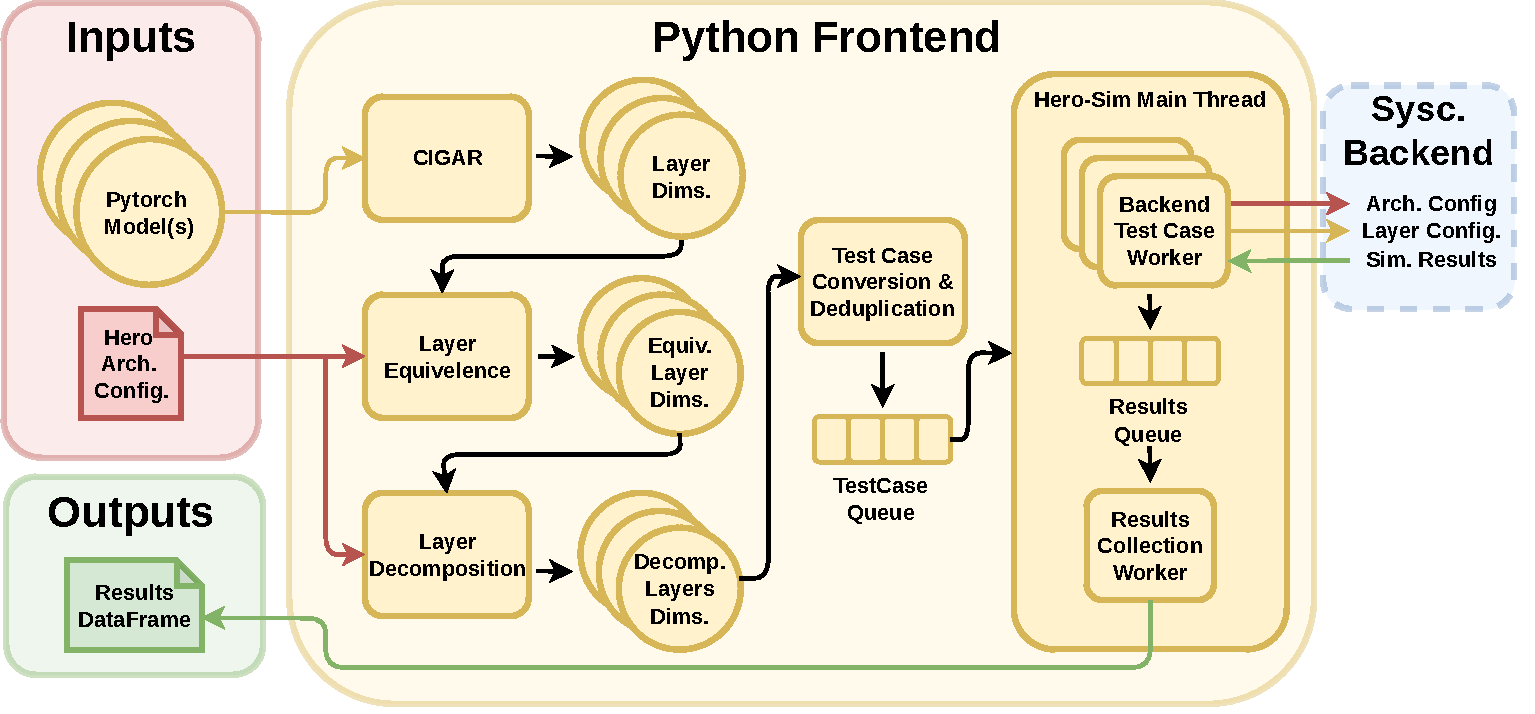
\includegraphics[scale=0.58]{fig/hero-sim-frontend.pdf}
    \caption{Hardware Implementation Taxonomy adapted from \cite{maestro}}
    \label{fig:hw_taxonomy}
\end{figure}


\subsection{SystemC backend}
\label{chap:hero:sim_platform:cigar_side}

Inputs outputs
initialization stages
handling dram interaction
metrics collected
validation

\begin{figure}[ht]
    \centering
    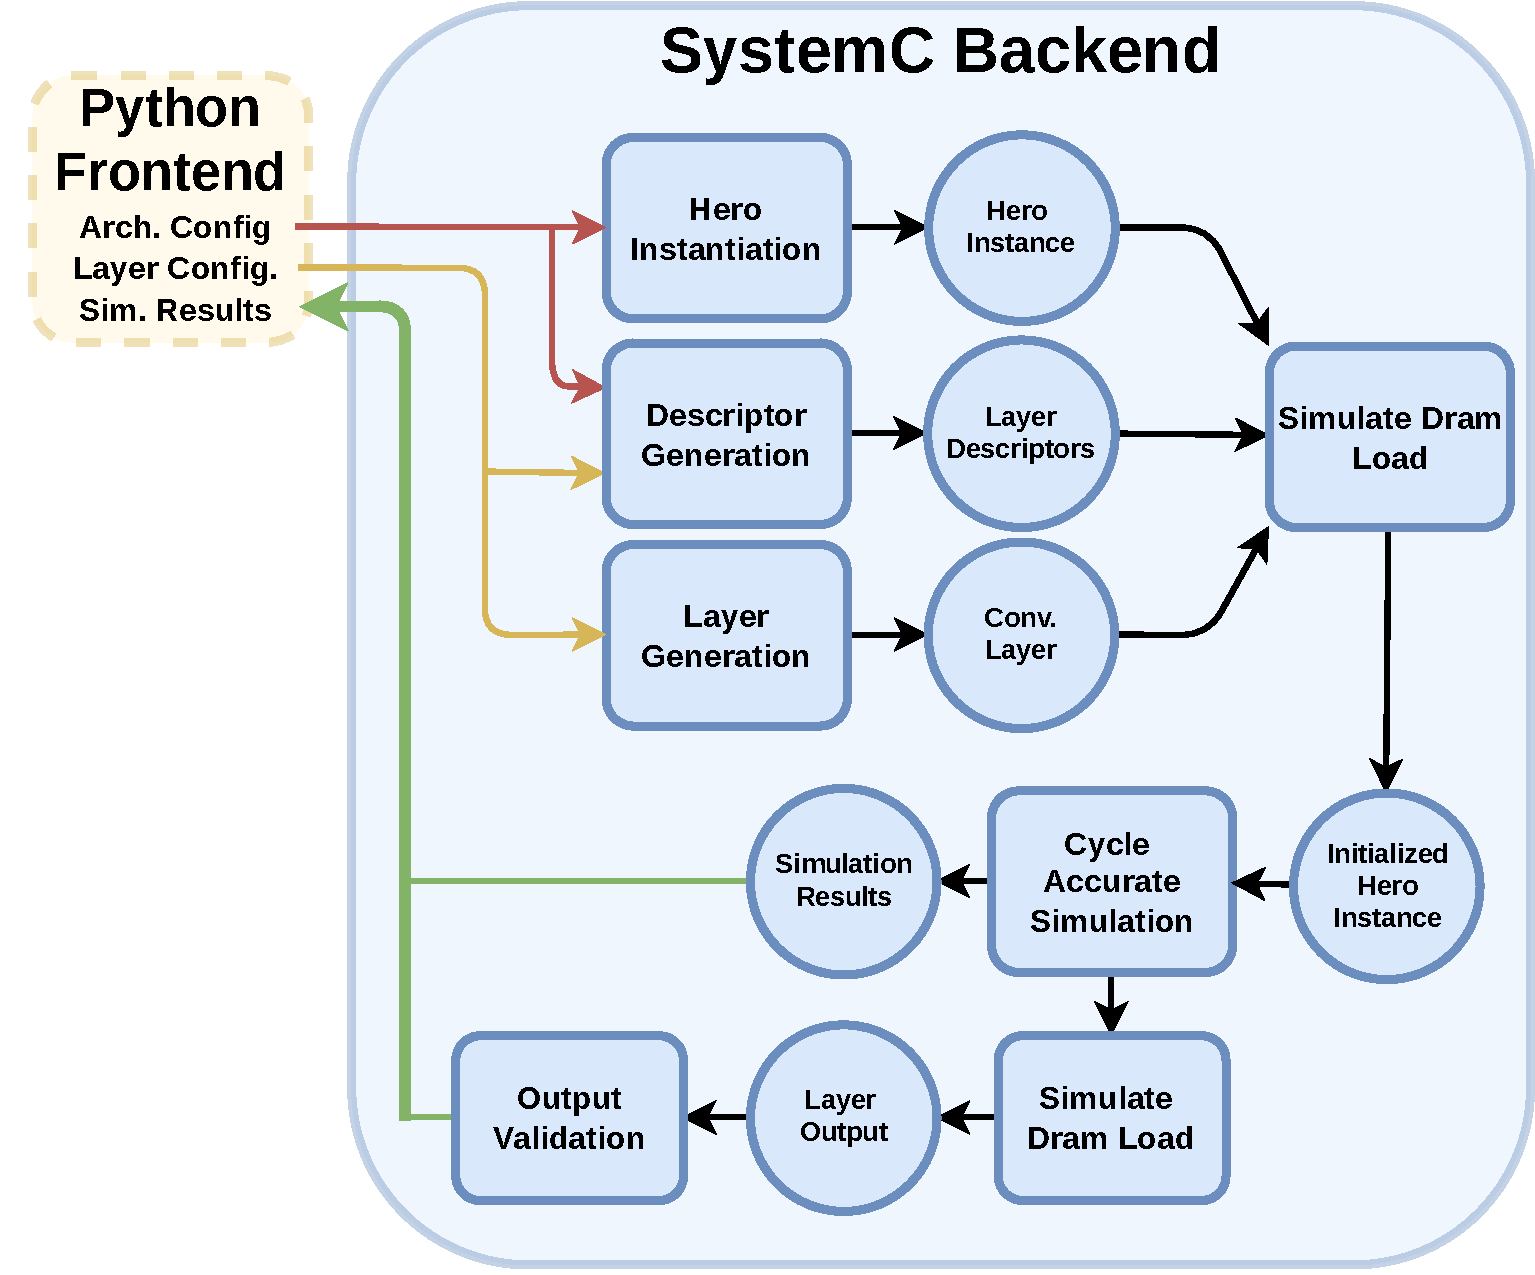
\includegraphics[scale=0.58]{fig/hero-sim-backend.pdf}
    \caption{Hardware Implementation Taxonomy adapted from \cite{maestro}}
    \label{fig:hw_taxonomy}
\end{figure}

\section{Experimental Results}
\label{chap:hero:sim_platform:cigar_side}

CPU baseline
arch config simulated
To support as much as 85\% of convolution layers in TIMM
without requiring layer decomposition (to be discussed in
\autoref{chap:net_compile}) we only need to allocate 1 MB of storage for IFmap
memory (L3) and Ofmap memory in either of the HERO architectures presented in
\autoref{chap:dda:hw_dse:final}.
\begin{table}[]
    \center
    \begin{tabular}{|l|l|}
    \hline
    Data Element Type & On-Chip Storage    \\ \hline
    Weights           & N/A   \\ \hline
    IFmap L3          & $2^{20}$   \\ \hline
    IFmap L2          & $2^{9}$   \\ \hline
    OFmap             & $2^{20}$   \\ \hline
    \end{tabular}
    \caption{Assumed on-chip storage for different data elements in a convolution operation}
    \label{tab:assumed_storage}
\end{table}


% # Config
% arch_config
% "filter_count": 32,
% "channel_count": 18,
% "directly_supported_kernels": [(1, 1), (3, 3)],
% "ifmap_mem_ub": 2**20 // 18 * 18,
% "allow_ifmap_distribution": True,
% "ofmap_mem_ub": 2**20,
% "allow_ofmap_distribution": True,
% "reuse_chain_bank_size": 512,
% "weight_bank_size": 16,
% "groups_supported": False,

assumed clk speed = 1Ghz
assumed precisions of weights and featuremaps
assumed rescaling when transfering back ofmaps (need to find citation)

\subsection{Percent of network compute for supported layers}
\label{chap:hero:sim_platform:cigar_side}

layers supported represent a substantial amount of total compute by network
how do I compute that since ops may be hard to estimate for some layers?
using runtime

\begin{figure}[ht]
    \centering
    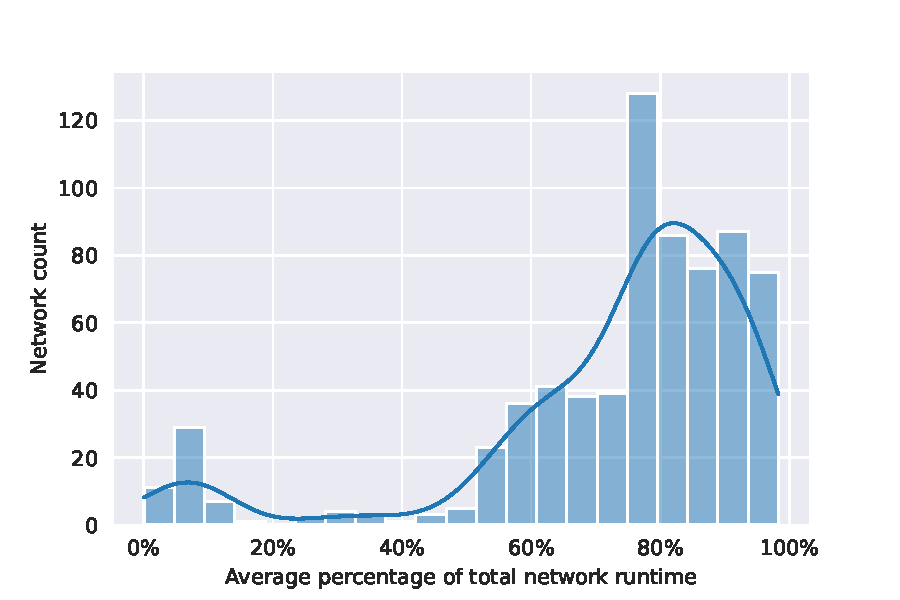
\includegraphics[scale=0.58]{Plots/overview/percent.pdf}
    \caption{Hardware Implementation Taxonomy adapted from \cite{maestro}}
    \label{fig:hw_taxonomy}
\end{figure}

\subsection{Latency and Speedup over CPU Baseline}
\label{chap:hero:sim_platform:cigar_side}

most networks/ layers benefit
median network speedup over 

\begin{figure}[ht]
    \centering
    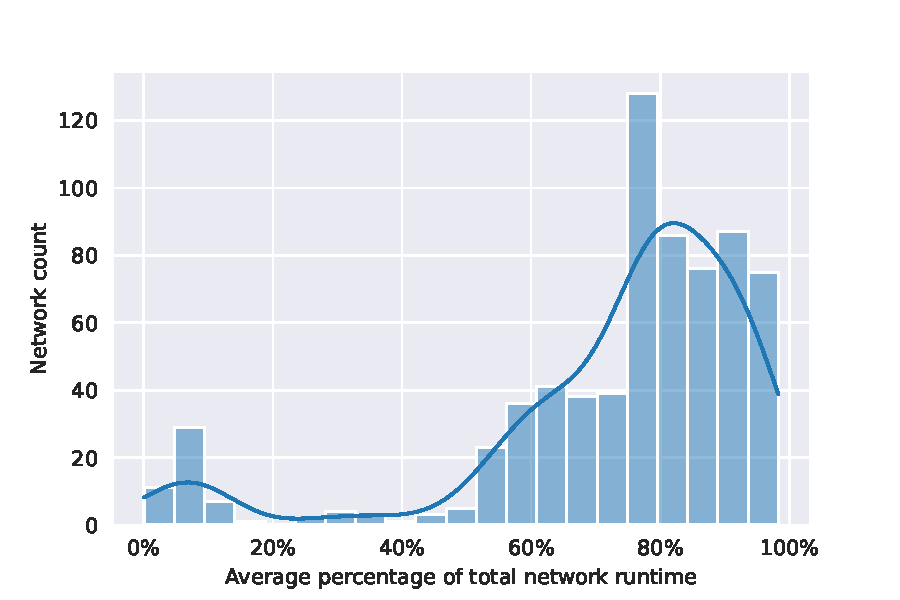
\includegraphics[scale=0.58]{Plots/overview/percent.pdf}
    \caption{Hardware Implementation Taxonomy adapted from \cite{maestro}}
    \label{fig:hw_taxonomy}
\end{figure}

Some networks don't benefit

\begin{figure}[ht]
    \centering
    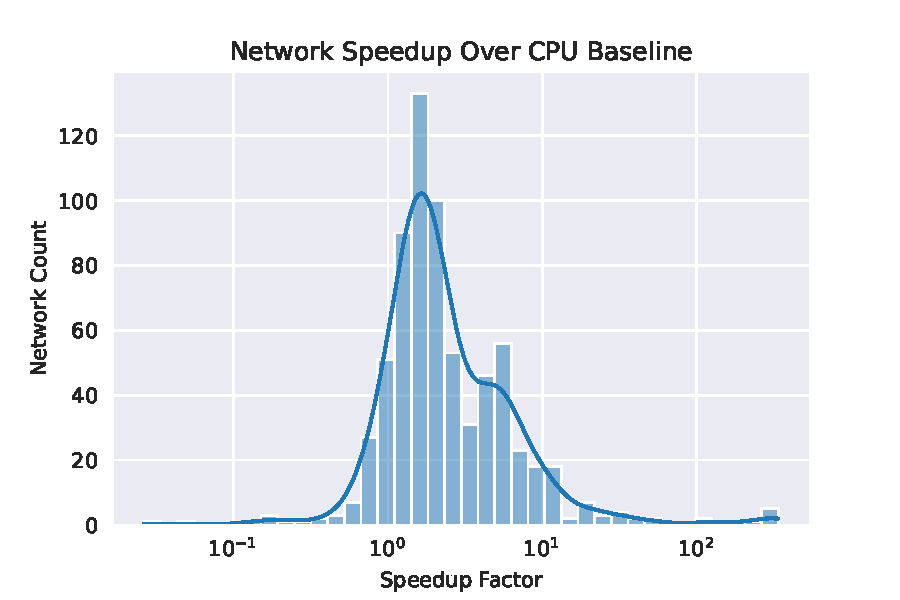
\includegraphics[scale=0.58]{Plots/latency/net_speedup.pdf}
    \caption{Hardware Implementation Taxonomy adapted from \cite{maestro}}
    \label{fig:hw_taxonomy}
\end{figure}

12\% of layers don't benefit

\begin{figure}[ht]
    \centering
    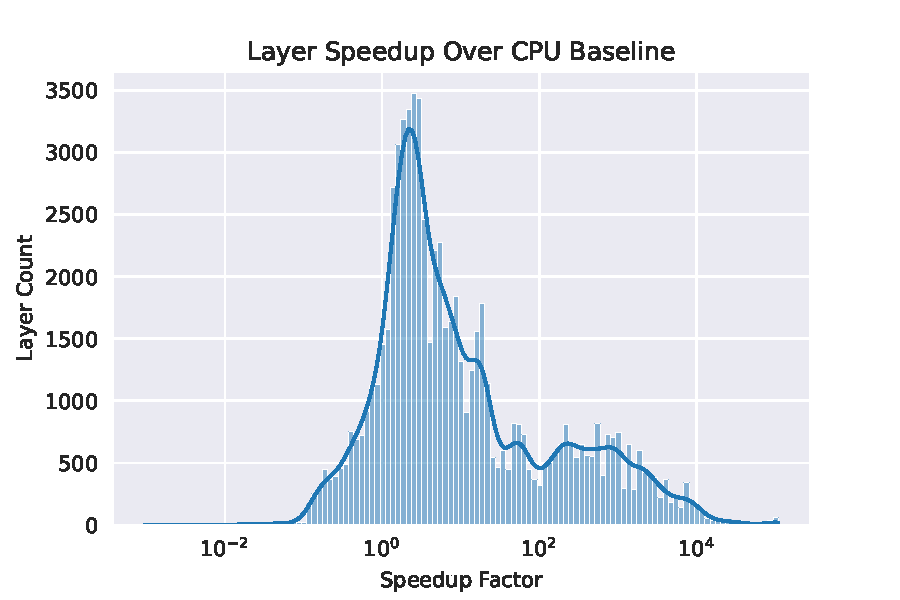
\includegraphics[scale=0.58]{Plots/latency/layer_speedup.pdf}
    \caption{Hardware Implementation Taxonomy adapted from \cite{maestro}}
    \label{fig:hw_taxonomy}
\end{figure}


why? see utilization
here's a boxplot of per layer speedup excluding layers with no speedup

\begin{figure}[ht]
    \centering
    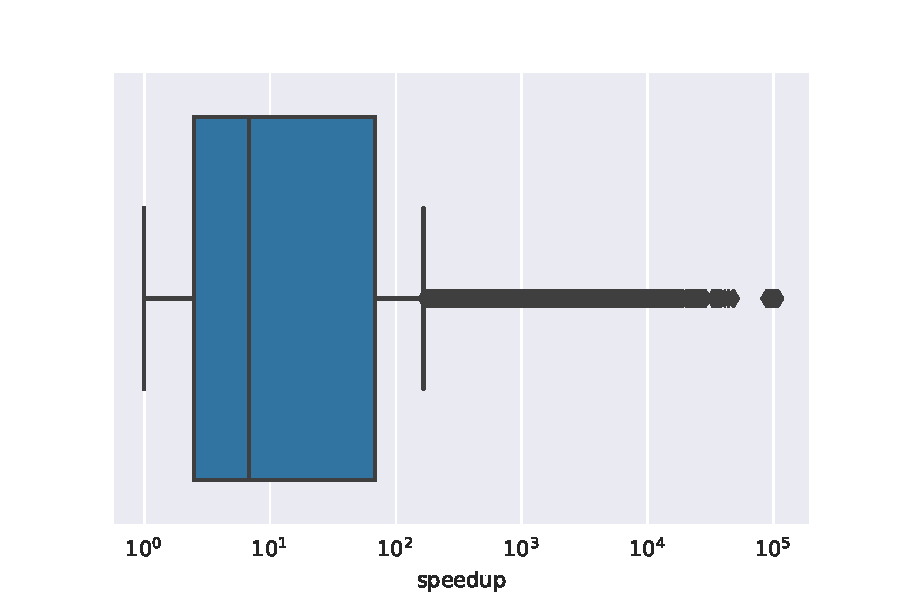
\includegraphics[scale=0.58]{Plots/latency/speedup_gt_1_boxplot.pdf}
    \caption{Hardware Implementation Taxonomy adapted from \cite{maestro}}
    \label{fig:hw_taxonomy}
\end{figure}

estimated fps based on supported layers, note that this should be taken as upper
bound because unsupported supported layers may take up more of the runtime than
anticipated (references earlier figure)

\begin{figure}[ht]
    \centering
    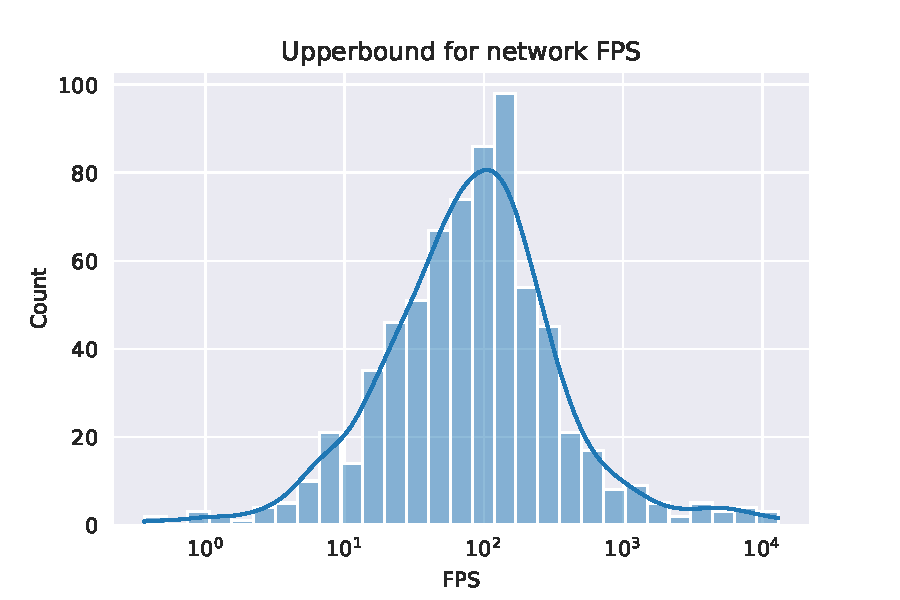
\includegraphics[scale=0.58]{Plots/latency/fps.pdf}
    \caption{Hardware Implementation Taxonomy adapted from \cite{maestro}}
    \label{fig:hw_taxonomy}
\end{figure}


\subsection{Utilization}
\label{chap:hero:sim_platform:cigar_side}

utilization is a surrogate for how well layers map to the architecture
some networks benefit substantially from the architecture
others don't. 

network level distribution of utilization is generally flat with
about a third not benefiting enough from the architecture due to low
utilization. 


\begin{figure}[ht]
    \centering
    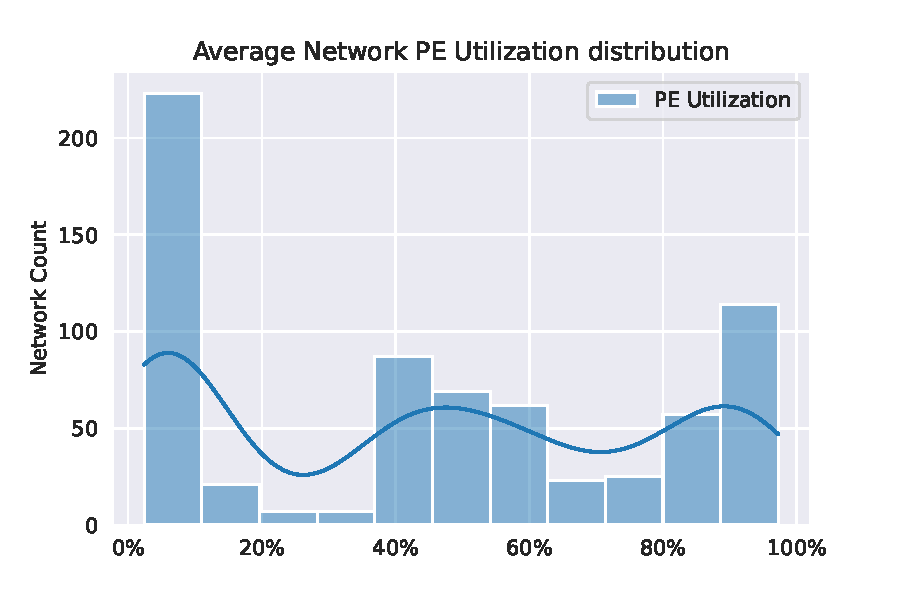
\includegraphics[scale=0.58]{Plots/utilization/network.pdf}
    \caption{Hardware Implementation Taxonomy adapted from \cite{maestro}}
    \label{fig:hw_taxonomy}
\end{figure}


At a more granular level it seems like utilization is bimodal

\begin{figure}[ht]
    \centering
    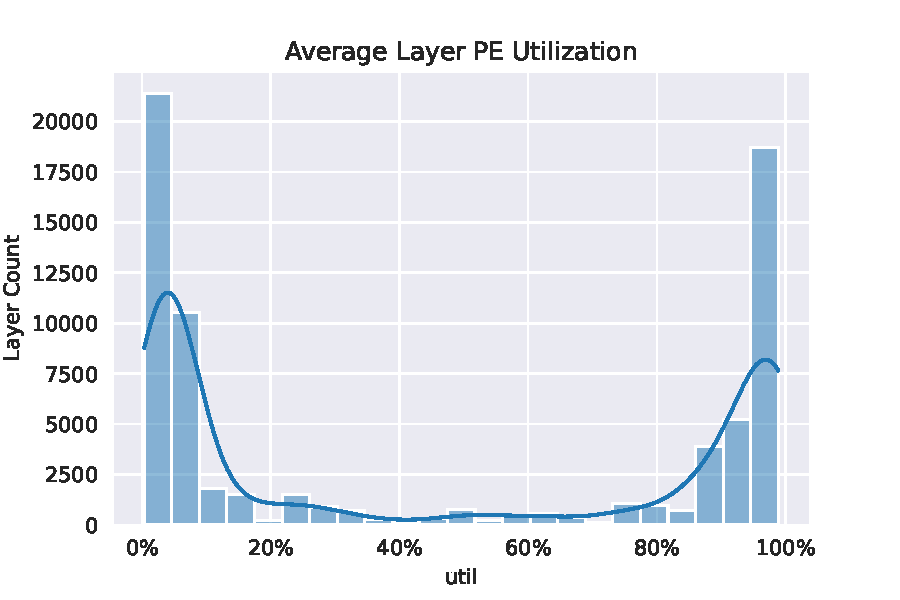
\includegraphics[scale=0.58]{Plots/utilization/layers.pdf}
    \caption{Hardware Implementation Taxonomy adapted from \cite{maestro}}
    \label{fig:hw_taxonomy}
\end{figure}

if utilization is low for small layers that would make sense
plotting utilization vs macs we see that we see that generally there's a trend where low
utilization correlates with lower macs
but there is a bulge MACS where high Macs correlates
with low utilization. Why? 

\begin{figure}[ht]
    \centering
    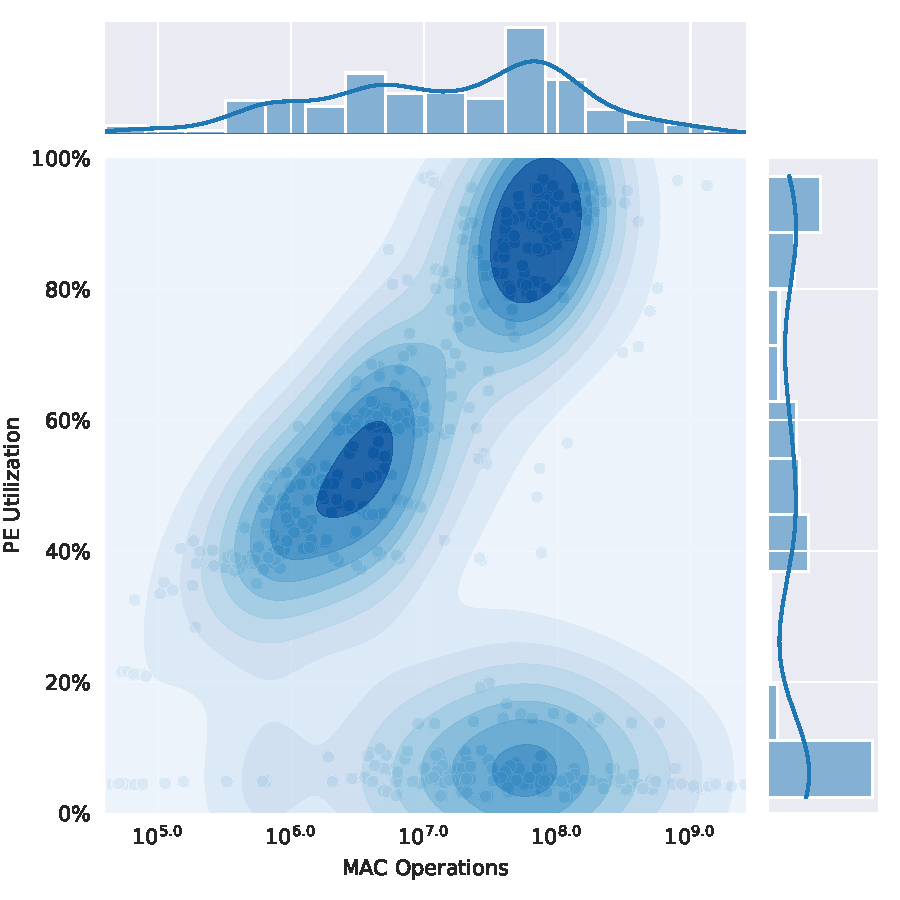
\includegraphics[scale=0.58]{Plots/utilization/util_vs_macs.pdf}
    \caption{Hardware Implementation Taxonomy adapted from \cite{maestro}}
    \label{fig:hw_taxonomy}
\end{figure}


Maybe layer decomposition and on chip memory plays a role here
Scatter plot of layers with speedup < 1 

\begin{figure}[ht]
    \centering
    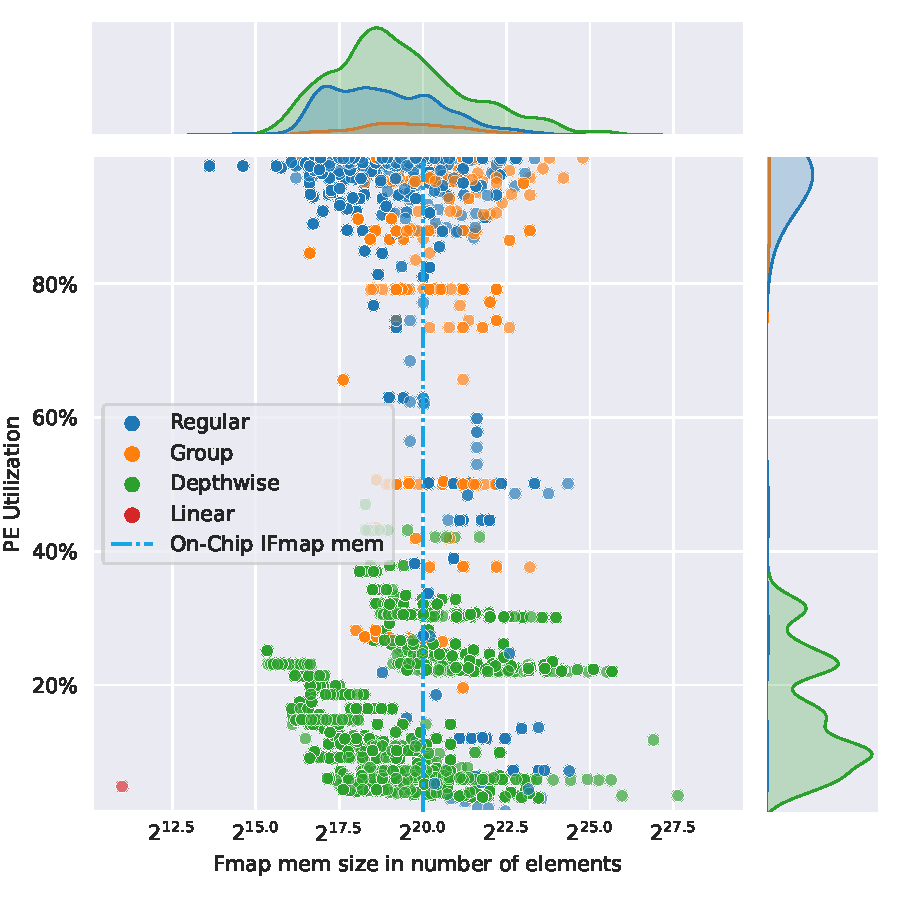
\includegraphics[scale=0.58]{Plots/utilization/util_vs_fmap.pdf}
    \caption{Hardware Implementation Taxonomy adapted from \cite{maestro}}
    \label{fig:hw_taxonomy}
\end{figure}


Misteriously theres  a cluster of layers with high utilization and low speedup
they fall on bouth sides of the on-chip memory line

If we look at types of layers that have low util and low speedup they're all
depthwise layers which are decomposed by group and poorly map to the
architecture

\begin{figure}[ht]
    \centering
    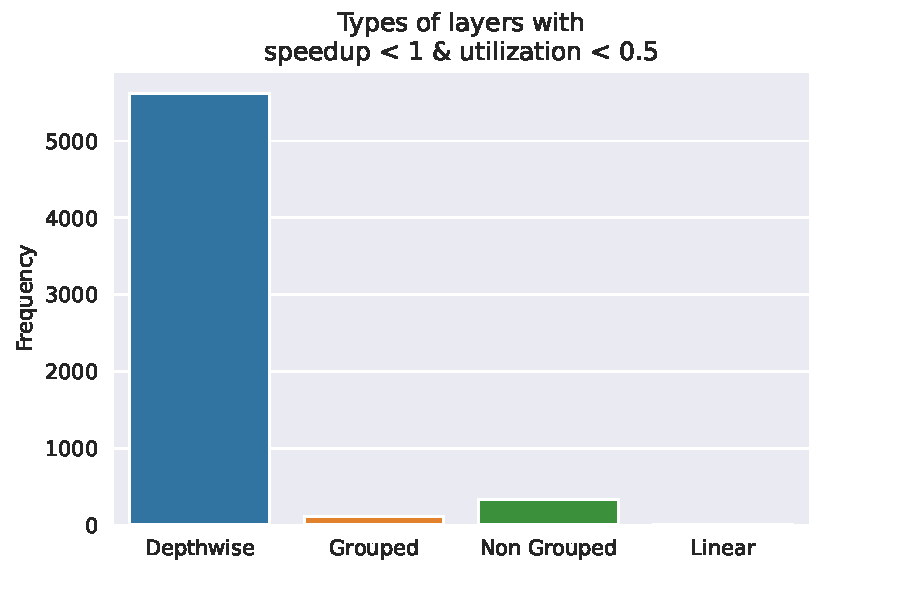
\includegraphics[scale=0.58]{Plots/utilization/type_of_low_util.pdf}
    \caption{Hardware Implementation Taxonomy adapted from \cite{maestro}}
    \label{fig:hw_taxonomy}
\end{figure}


If we look at layers with large footprint and low speedup they're size limits
concurrency because the full throughput of on-chip memory can't be used, these
layers need us to exploit a different kind of concurrency other than F, C Ky and
KX

\begin{figure}[ht]
    \centering
    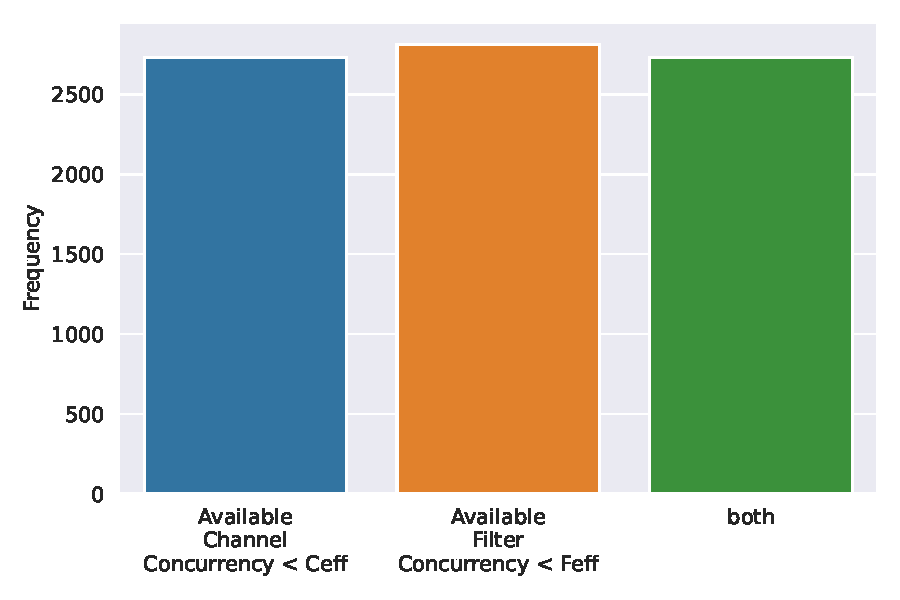
\includegraphics[scale=0.58]{Plots/utilization/low_util_big_fmap.pdf}
    \caption{Hardware Implementation Taxonomy adapted from \cite{maestro}}
    \label{fig:hw_taxonomy}
\end{figure}

what about layers with high utilization but low speedup
Not enough PES because of some many channels and filters


\begin{figure}[ht]
    \centering
    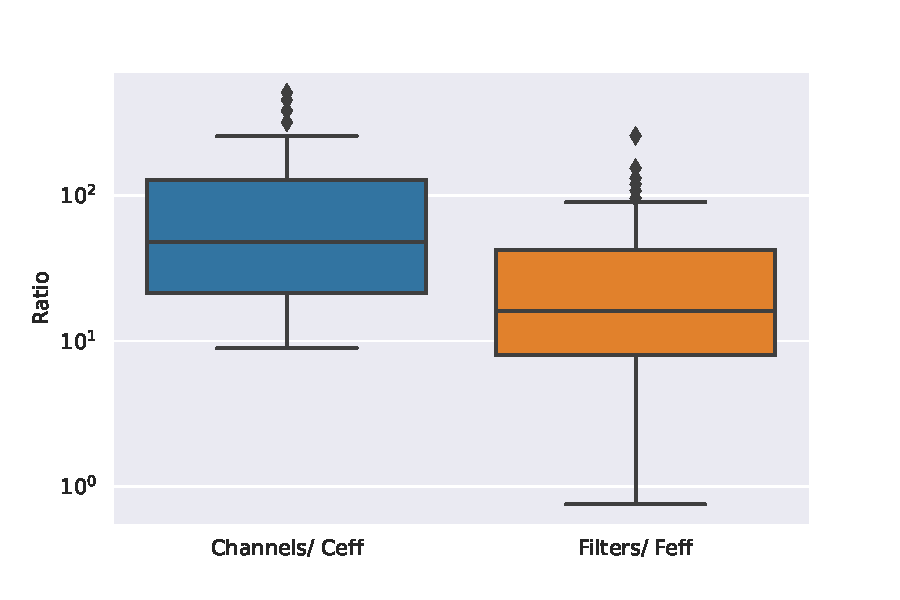
\includegraphics[scale=0.58]{Plots/utilization/ratios.pdf}
    \caption{Hardware Implementation Taxonomy adapted from \cite{maestro}}
    \label{fig:hw_taxonomy}
\end{figure}

summary barplot

\begin{figure}[ht]
    \centering
    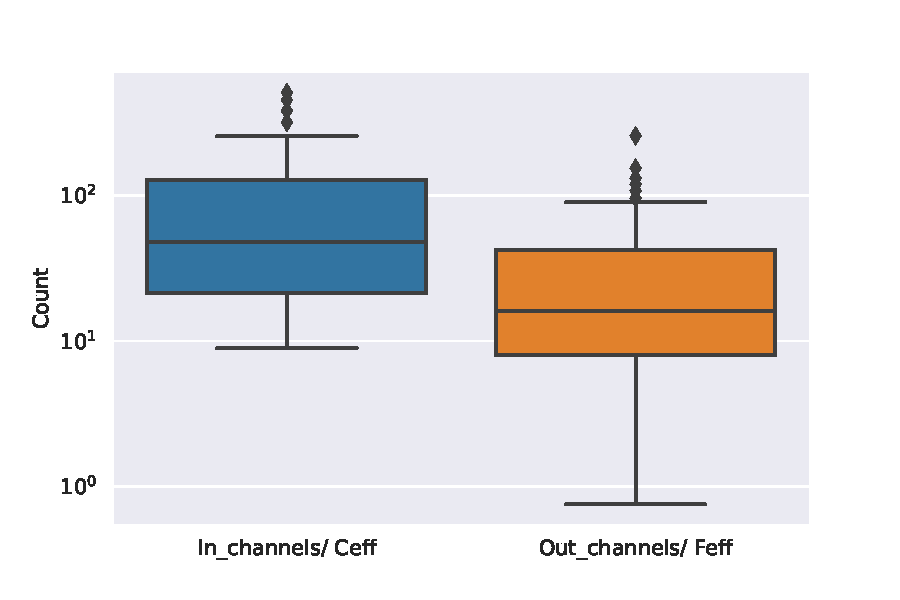
\includegraphics[scale=0.58]{Plots/utilization/summary.pdf}
    \caption{Hardware Implementation Taxonomy adapted from \cite{maestro}}
    \label{fig:hw_taxonomy}
\end{figure}


\subsection{DRAM Bandwidth}
\label{chap:hero:sim_platform:cigar_side}

network and layer bandwidth histograms
within ddr4 spec

\begin{figure}[ht]
    \centering
    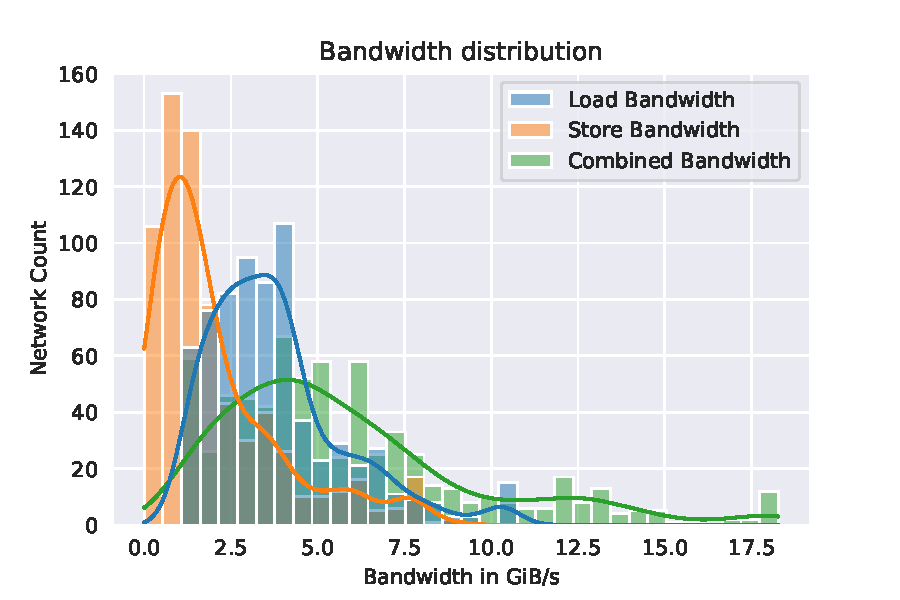
\includegraphics[scale=0.58]{Plots/resources/net_bw.pdf}
    \caption{Hardware Implementation Taxonomy adapted from \cite{maestro}}
    \label{fig:hw_taxonomy}
\end{figure}


\subsection{Energy}
\label{chap:hero:sim_platform:cigar_side}

used energy model in cite energy model
add energy model as table


mac is basically free
dram dominates
network inferences/ j median is around 57
excluding dram number jumps to 20K
there's room to reduce on-chip data movement by exploiting different kinds of
concurrency

\subsection{Area}
\label{chap:conv_gemm_equiv:overhead}

area model as table
bulk goes to ofmap storage and ifmap storage
ofmap storage requires higher precision

\subsection{Descriptor program scaling}
\label{chap:hero:sim_platform:cigar_side}

median required storage for descriptors per address generator is around 100
scaling can be improved with more complicated descriptors

\subsection{Per network results}
\label{chap:hero:sim_platform:cigar_side}

networks chosen
resnet50 (popular and backbone for alot of other networks)
mobilenetv3 specific to edge devices and has depthwise layers (let's see effect
of offloading on cpu)
hrnet18 flexible network used for variety of tasks, also has larger layers
